\renewcommand{\theequation}{\theenumi}
\begin{enumerate}[label=\thesubsection.\arabic*.,ref=\thesubsection.\theenumi]
\numberwithin{equation}{enumi}

\item \solution The general of a circle equation is $Ax^2 + Bxy + Ay^2 + Dx + Ey + F$, the equation can be represented as follow in the vector form:
\begin{align}
x^T 
\begin{pmatrix}
A & \frac{B}{2} \\
\frac{B}{2} & A
\end{pmatrix}
x + 
\begin{pmatrix}
D & E 
\end{pmatrix}
x + F = 0
\end{align}

\item To find the center - $\vec{O}$ and radius - $r$ of a circle:
\begin{align}
\vec{O} &= \frac{-1}{2A}\begin{pmatrix}
D & E 
\end{pmatrix}\label{eq:circle_example3}\\
r &= \frac{1}{A}\sqrt{ \frac{1}{4} \| \myvec{D\\ E}\ \|^2 - F^2}\label{eq:circle_example4}
\end{align}

\item The values given:
\begin{align}
A &= 1\\
D &= 8 \\
E &= 10 \\
F &= -8
\end{align}

\item Substituting the values in equation \ref{eq:circle_example3} and \ref{eq:circle_example4}:
\begin{align}
\vec{O} &= \myvec{-4\\-5}\\
r &= 7
\end{align} 

\item 
\begin{figure}[!ht]
\centering
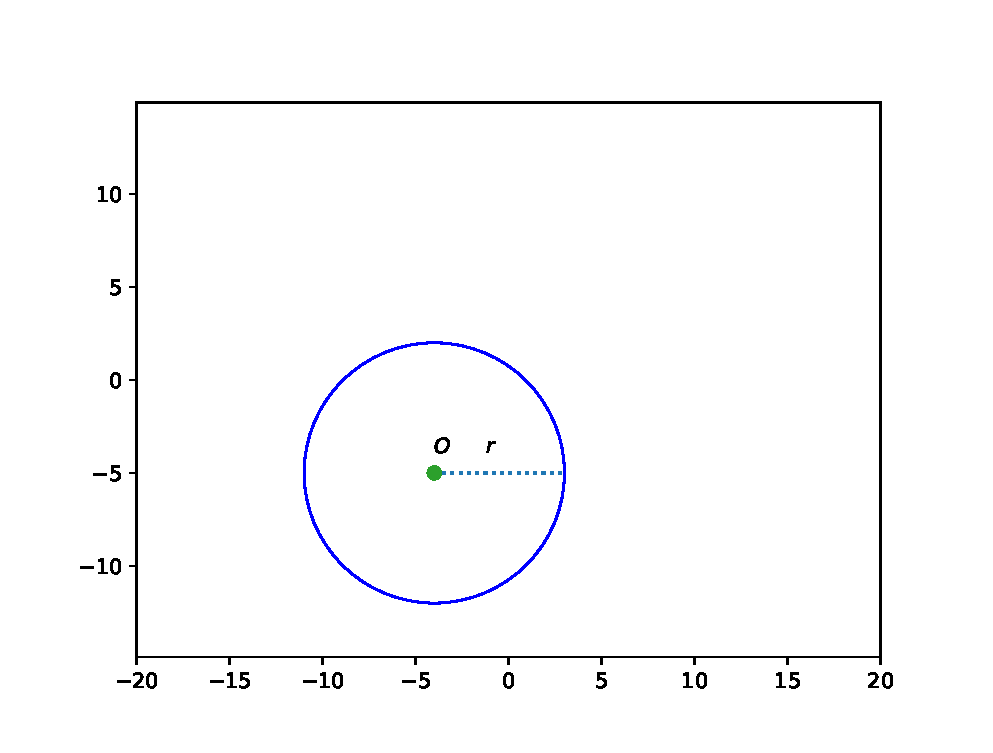
\includegraphics[width=\columnwidth]{./figs/circle_examp/circle.eps}
\caption{Circle generated using python}
\label{fig:circle2_circle_examp}
\end{figure} 

The following Python code generates Fig. \ref{fig:circle2_circle_examp}

\begin{lstlisting}
codes/circle_exam.py
\end{lstlisting}

\end{enumerate}